\noindent
\section{Analyzing reviewer tendencies}
\label{reviewer}
%\mycheckng{What percentage of reviewers are anomalous}
Reviewers are assigned with the responsibility of judging the quality of a submitted paper and hence their knowledge and training is highly critical. 
In fact, the decision of acceptance or rejection of a paper depends on the reviewer's perception of the paper. 

%\begin{figure}
% \centering
% \includegraphics[scale = 0.26]{figures/reviewer.eps}
% \caption{\label{reviewer} Cumulative distribution function of fraction of cases a reviewer was a part of a multi-referee system across all the reviewers
% for both JHEP and JSTAT datasets.}
%\end{figure}



%We calculate for each reviewer the fraction of cases where he is a part of a multi-referee set among his total assignments and plot the 
%cumulative distribution function of this fraction in figure~\ref{reviewer} for both JHEP and JSTAT datasets. The figure clearly indicates 
%that for JHEP the reviewers are mostly part of a single-referee set up while for JSTAT, the reviewers are part of a multi-referee set up in many more cases. 

% \begin{figure} 
%  \centering
%  \includegraphics[scale = 0.26]{figures/ed_ref_comb.eps}
%  \caption{\label{reviewer} Cumulative distribution function of the fraction of cases a reviewer is a part of a multi-referee system across all the reviewers for JHEP and JSTAT datasets.}\end{figure}
\begin{figure}
 \centering
 \includegraphics[scale = 0.3]{./texfiles/Chapter_4/cikm_17/figures/citation_delay_acpt_ratio_jhep.eps}
 \caption{\label{a_d_jhep} Mean citation versus (a) accept ratio (b) assignment delay buckets for the JHEP dataset. 
 Note that the papers are segregated into accept ratio/delay bins and the mean citation is calculated for each bin. 
 Typical bin sizes for accept ratio are $<0.1$,$(\geq 0.1$ and $<0.2)$ and so on while for delay the sizes are $<100$, $(\geq 100$ and $< 200)$ and so on.}
\end{figure}

%We further leverage the technique introduced in~\cite{sikdar2016anomalies} and identify the set of under-performing
% reviewers for both the datasets. 
% \mycheck{put in the definition of underperforming/anomalous-----}
In~\cite{sikdar2016anomalies} authors define a referee/editor to be anomalous (under-performing) if - \\
(i) papers accepted by him/her have low citation (research wrongly judged to be impactful)\\
(ii) papers rejected by him/her have high citation (quality research wrongly judged as flawed)\\
In fact, the authors propose a method for identifying under-performing (anomalous) referees/editors. Leveraging on the same method we observe that  
 the proportion of referees classified as under-performing are approximately $26\%$ and $21\%$ respectively for JHEP and JSTAT datasets.
%The authors hypothesize that accepted papers receiving low citation as well as rejected papers receiving high citations are anomalous cases as 
%ideally they should have been respectively rejected and accepted.  
We make the following general observations - \\
(i) If we consider all the cases where an under-performing editor assigned multiple reviewers for a submission, in $69.8\%$ cases 
at least one of them was under-performing. This indicates that unless the reviewers are selected carefully, chances are it might lead to wrong judgment.\\
(ii) Under-performing reviewers when part of a multi-referee system tend to do a better judgment as compared to cases when they serve as single reviewers.
This is illustrated by the fact that average citation of the accepted  papers reviewed by multiple reviewers with at least one under-performing reviewer ($32.4$) 
is more compared to that of the papers reviewed by a single anomalous reviewer ($18.2$) across the two datasets.
%\vspace{-4mm}
\subsection{Factors determining performance of the referees}
We next look into factors that could be used to quantify the performance of the reviewers. The quantification can be used as a 
fitness value for assignment of a new submission (we use these to calculate these quantities in a later section to develop a scheme for automatic referee group selection). 
Given a submission, we identify two factors that are indicative of reviewer fitness (i) accept ratio and (ii) time since the last assignment.\\
\noindent(i) \textit{Accept ratio}: Given a submission, we consider for each reviewer ($i$) the fraction of papers (s)he has accepted at the time of submission. 
We denote this by $a_i$. To show that it is indeed an indicator we consider all the accepted and the rejected papers as well as their assigned reviewers. 
We then calculate the accept ratio of the assigned reviewers and compare them against the citations received by each of them. 
In figures~\ref{a_d_jhep}(a) (JHEP) and~\ref{a_d_jstat}(a) (JSTAT) we plot accept ratio against the citations received by the accepted as well as the rejected papers. 
Note that we bin the papers based on the accept ratio and calculate the average citation in each case. The typical bin sizes are $\leq 0.1$, $(> 0.1$ and $\leq 0.2)$ and so on. 
We hence obtain $10$ such bins numbered 1-10. 
In case of multi-referee papers the average accept ratio of the reviewers is considered. We observe that for both the datasets very high accept ratio or a very low accept 
ratio might lead to wrong judgment. \\ 
\noindent(ii) \textit{Time since last assignment}: Given a submission and its corresponding submission date we calculate for each reviewer ($i$) the time (in days) between the 
last review assignment date and the submission date (denoted by $d_i$). To illustrate the rationale, we again consider all the accepted and the rejected papers and calculate 
the delay for the assigned reviewers. We again bin the delay values and calculate the average citation (refer to figures~\ref{a_d_jhep}(b) and~\ref{a_d_jstat}(b)). Typical bin 
sizes are $\leq 100$, $(> 100$ and $\leq 200)$ and so on (10 such bins are obtained numbered 1-10). We observe that the reviewers who are assigned very close to their last 
assignment or those who have not been assigned for a long time often fail to correctly judge the quality of the paper correctly as the papers accepted by them are cited less 
on average while those rejected are cited more. 


% \begin{figure}
%  \centering
%  \includegraphics[scale = 0.26]{figures/citation_delay_acpt_ratio_jhep.eps}
%  \caption{\label{a_d_jhep} Mean citation versus (a) accept ratio (b) assignment delay buckets for the JHEP dataset. 
%  Note that the papers are segregated into accept ratio/delay bins and the mean citation is calculated for each bin. 
%  Typical bin sizes for accept ratio are $<0.1$,$(\geq 0.1$ and $<0.2)$ and so on while for delay the sizes are $<100$, $(\geq 100$ and $< 200)$ and so on.}
% \end{figure}

\begin{figure}
 \centering
 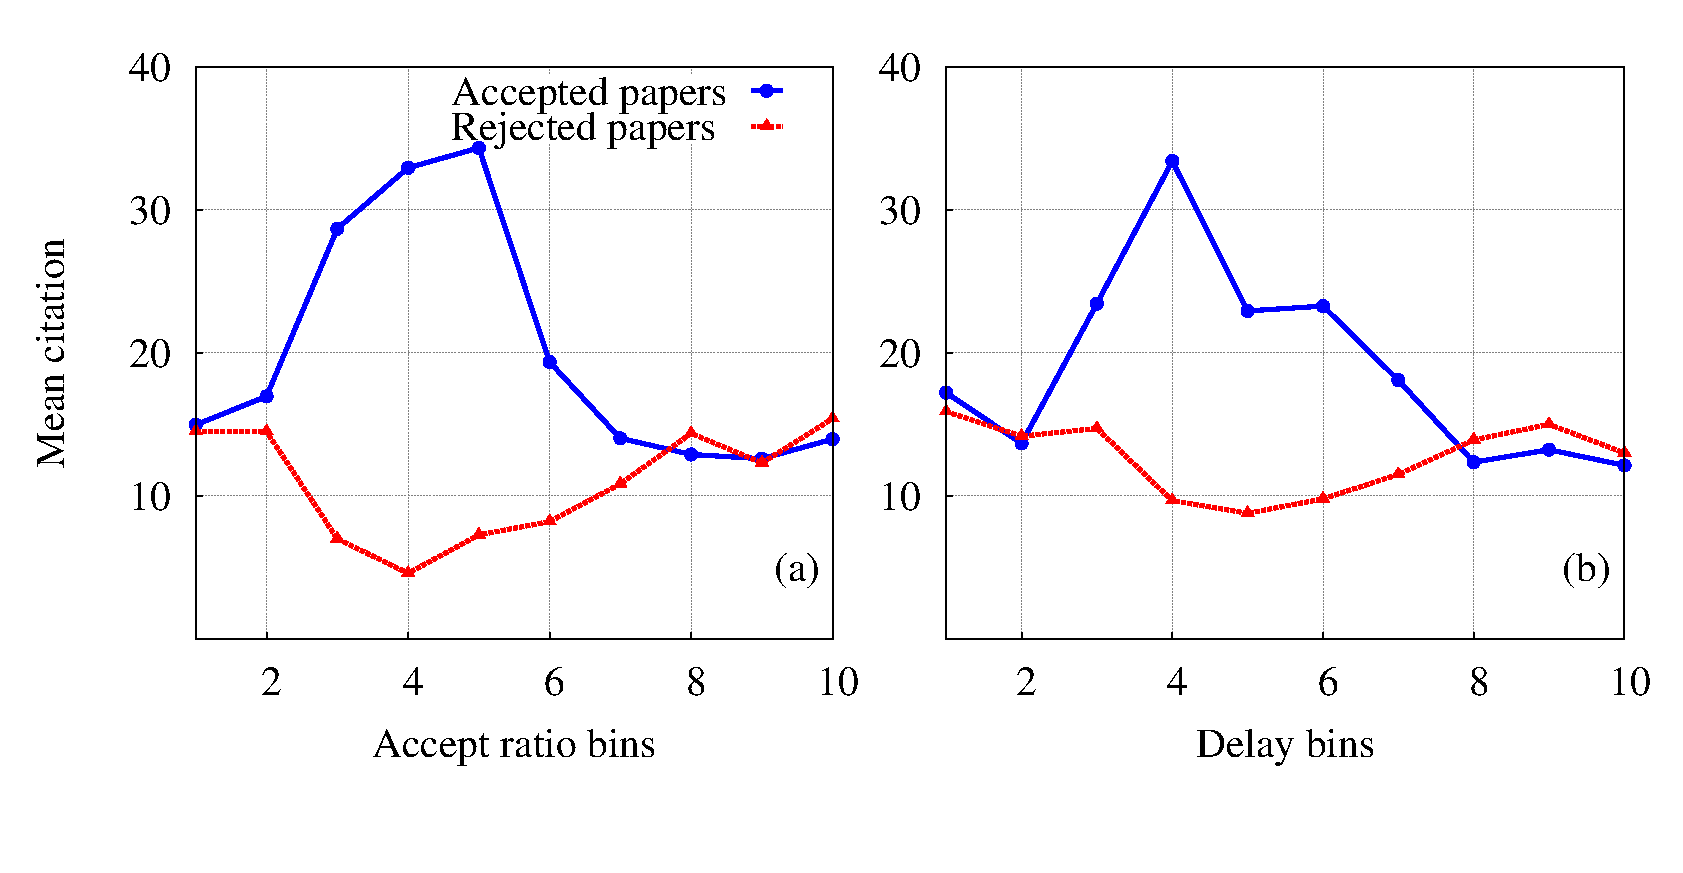
\includegraphics[scale = 0.3]{./texfiles/Chapter_4/cikm_17/figures/citation_delay_acpt_ratio_jstat.eps}
 \caption{\label{a_d_jstat} Mean citation versus (a) accept ratio (b) assignment delay buckets for JSTAT dataset. Note that the papers are 
 segregated into accept ratio/delay bins and the mean citation is calculated for each bin. Bin sizes are same as figure \ref{a_d_jhep}.}
\end{figure}


\subsection{Action with under-performing reviewers}
A naive solution could be to not assign the under-performing reviewers and only assign the best performing ones, but is not feasible 
since the number of referees is limited and they often decline assignments. Hence a better solution would be to group them such that the overall performance improves. 
To this aim, we first divide the reviewers into 3 classes separately for accept ratio and time 
since last assignment. A reviewer $i$ with accept ratio $a_i < 0.3$ is assigned ``Low'' (L), with $0.3 \leq a_i < 0.6$ is assigned ``Medium'' (M) and with $a_i \geq 0.6$ is 
assigned ``High'' (H). Note that reviewers in M were the best performing referees (refer to figures \ref{a_d_jhep}(a) and \ref{a_d_jstat}(a)). Each multi-refereed paper 
(by exactly 2 referees) is classified into one of the six classes (LL, MM, HH, LH, MH, LH) based on the class of each referee and the average citation of the papers in each 
class is noted (figure \ref{ref_perf}(a)). We observe that when both the referees belong to M class (MM) the performance is naturally well. More importantly, reviewers in L and H class 
perform better when paired with a referee from M class (even better than MM). On repeating the same experiment with time since last assignment, 
we observe a similar trend (figure \ref{ref_perf}(b)) with MM class performing the best followed by MH and LM.  
Note that in this case reviewers with $d_i < 100$ are assigned class L, with $100 \leq d_i < 300$ are assigned M and rest are assigned H. 
%This indicates that grouping 
%reviewers while assigning multiple referees for a 
%submission is highly critical toward improving the effectiveness of the system. 
%We further look into the proportion of discordant cases for each reviewer combination. 
More importantly the discordant cases mostly occur for 
class combinations LL, HH and LH (refer to table \ref{tab:dis}). In fact, MM has the least proportion of discordant cases. 
This further indicates the correct reviewer grouping is critical in curtailing the discordant cases which is one of the prime reasons behind the multi-reviewer system failing. 
Note that the above results are obtained for JHEP dataset and a similar pattern is observed 
for JSTAT as well.

\begin{figure}
 \centering
 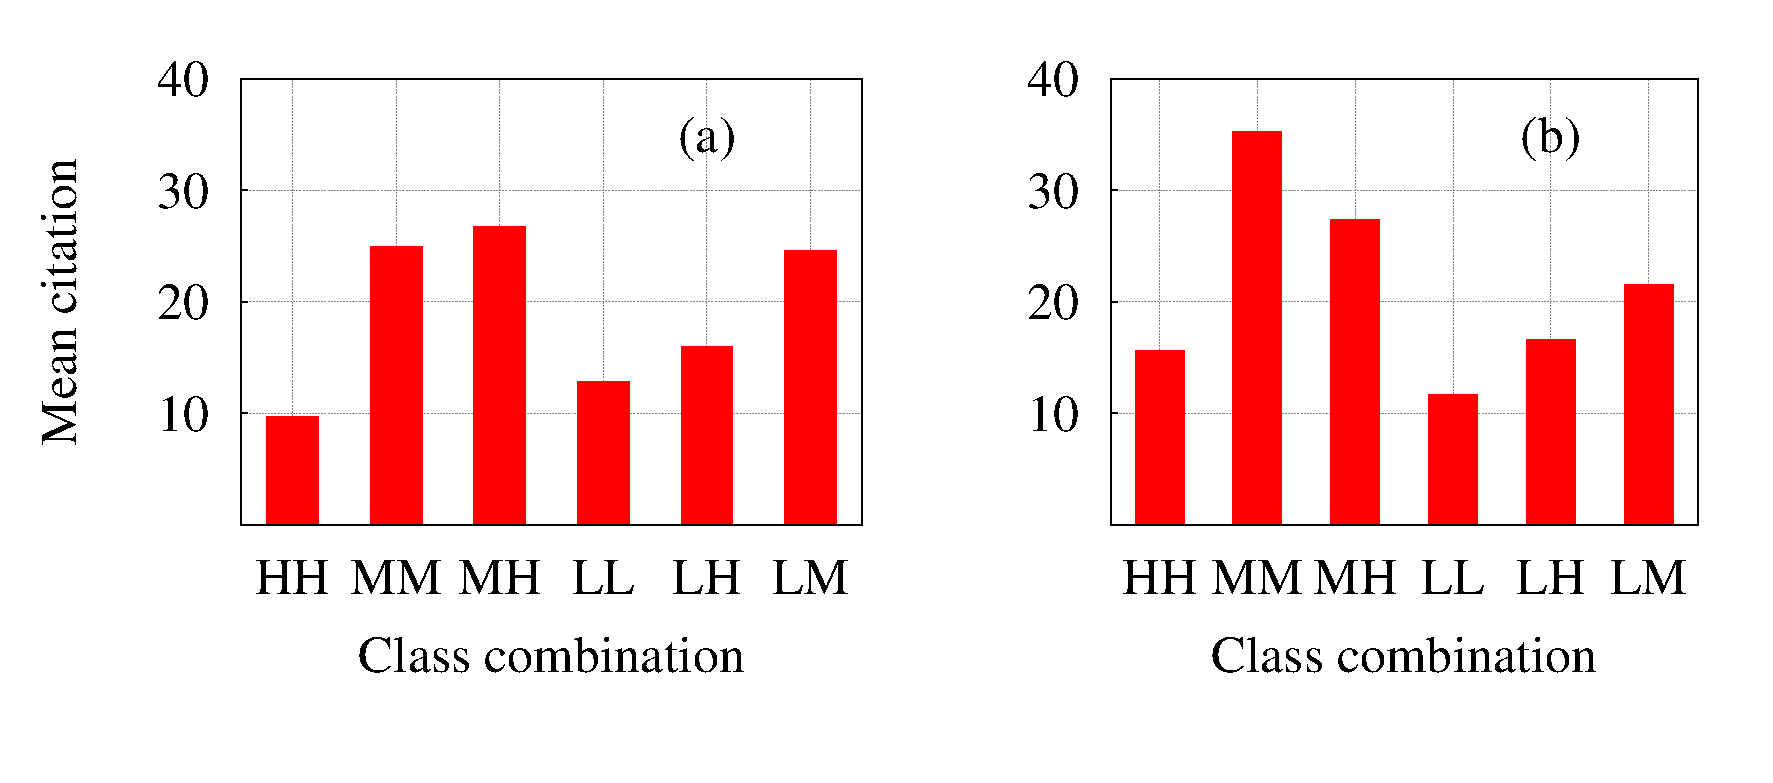
\includegraphics[scale = 0.3]{./texfiles/Chapter_4/cikm_17/figures/ref_performance.eps}
 \caption{\label{ref_perf} Mean citation for papers belonging particular class combination with respect to (a) accept ratio (b) time since last assignment. For example LL would represent a paper reviewed by referees both 
 belonging to class L.}
\end{figure}



\begin{table}
\centering
\caption{Proportion of discordant cases (length, sentiment and content) in each reviewer class combination with respect to (accept ratio, time since 
last assignment). }
\label{tab:dis}
\begin{tabular}{c|c|c|c}
\hline
           & Length       & Sentiment    & Content      \\ \hline
MM         & 0.176,0.159  & 0.194, 0.143 & 0.164, 0.152 \\ 
LM, HM     & 0.173, 0.162 & 0.243, 0.192 & 0.237, 0.216 \\ 
LL, HH, LH & 0.312, 0.254 & 0.371, 0.286 & 0.293, 0.311 \\ \hline
\end{tabular} 
\end{table}



\medskip
